\section{Aggregazione di unità discotiche}
\subsection{Unità con simmetria $C_3$}\begin{frame}\frametitle{Unità con simmetria $C_3$}
  \vspace{-5pt}   \begin{columns}
\column{0.3\linewidth}    \begin{figure}{\centering{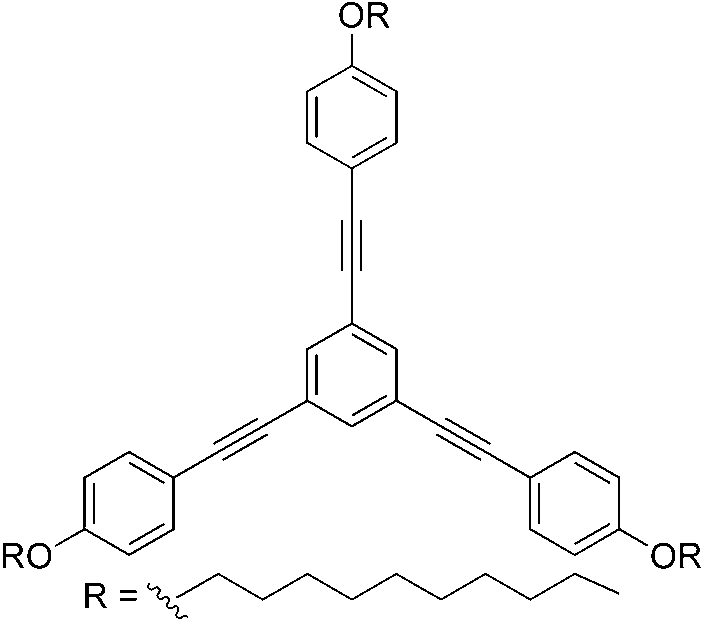
\includegraphics[width=0.8\textwidth]{sec2/alchino.png}}}\end{figure}    \column{0.3\linewidth} 
\begin{figure}{\centering{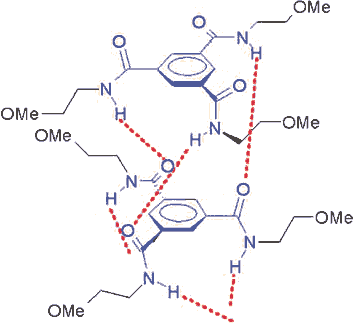
\includegraphics[width=0.8\textwidth]{sec2/C3legami.png}}}\end{figure}
 \column{0.3\linewidth} 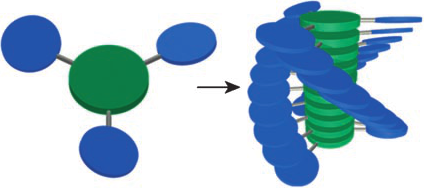
\includegraphics[width=1\textwidth]{sec2/C3.png}\end{columns}\vspace{15pt}
 
La conformazione elicoidale può esser causata da ingombro sterico (molecola a sinistra) o da nuovi legami ad idrogeno intermolecolari (molecola al centro). 


Variando le interazioni direzionali è possibile ottenere elicità controllate.

È \textbf{importante il bilancio delle interazioni}: 
troppe adirezionali diminuiscono l'ordinamento chirale indotto dalle direzionali.
             \end{frame}\logo{}
\subsection{Cooperatività}\begin{frame}\frametitle{Cooperatività}
   \begin{columns} \column{0.4\linewidth}La prima polimerizza cooperativamente.\begin{figure}{\centering{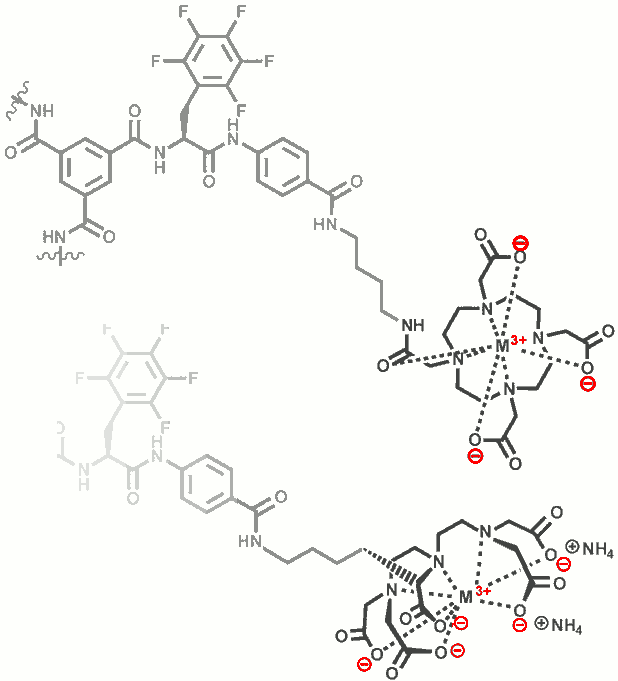
\includegraphics[width=1\textwidth]{sec2/anticoop.png}}}\end{figure} \column{0.6\linewidth} La motivazione è la presenza \textbf{nel dimero} dei \textbf{gruppi ammidici già orientati correttamente}.             \cite{tesi}
\begin{figure}{\centering{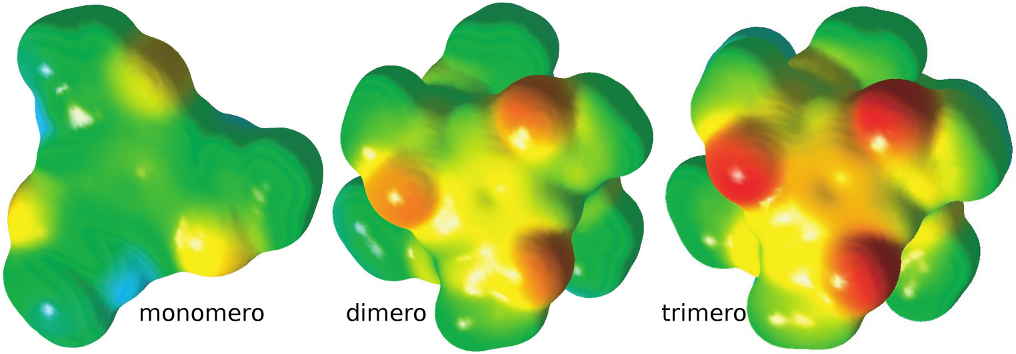
\includegraphics[width=0.7\textwidth]{sec2/1-2.png}}}\end{figure}
La seconda molecola ha polimerizzazione anticooperativa (controllo della dimensione). Alzando la forza ionica della soluzione diventa cooperativa. \cite{2}\end{columns}            
                                      \end{frame}\logo{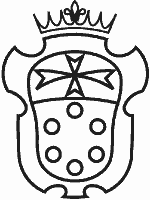
\includegraphics[width=0.07\paperwidth]{snslogo.png}}
\subsection{Amplificazione di chiralità}\subsubsection{Catene laterali}\begin{frame}\frametitle{Amplificazione di chiralità}\framesubtitle{Catene laterali}
L'interazione sterica tra catene laterali chirali può indurre un senso di rotazione preferenziale. \textbf{I monomeri non hanno CD} perciò misurazioni CD sono sensibili solo alla chiralità supramolecolare.\vspace{10pt}
\begin{columns}
\column{0.8\linewidth} \textbf{Effetto pari-dispari}: spostando di un carbonio il centro chirale si ha una inversione dei segni dei picchi al CD mantenendo lo stesso modulo, dunque un'inversione di rotazione dell'aggregato.\column{0.2\linewidth}\vspace{-20pt}\begin{figure}{\centering{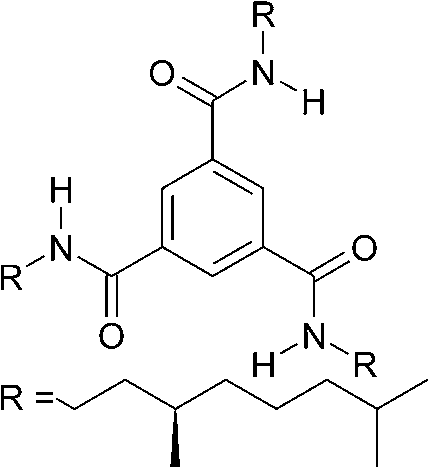
\includegraphics[width=1\textwidth]{sec2/C3semplice.png}}}\end{figure}\end{columns}\vspace{10pt} % \vspace{20pt}
\textbf{Se delle tre catene laterali solo una è chirale}, l'ellitticità in un omopolimero non varia. Invece la \textbf{penalità per errore puntuale diminuisce} (dunque l'ampl. chirale in esp. sergenti e soldati diminuisce ma aumenta in esp. regola di maggioranza). \cite{tesi}
\end{frame}
\logo{}
\subsubsection{Effetto della temperatura}\begin{frame}\frametitle{Amplificazione di chiralità}\framesubtitle{Effetto della temperatura}
L'\textbf{aumento della temperatura} provoca: \cite{tesi}
\begin{itemize}
 \item pol. omochirale CD\textdownarrow (a causa della \textbf{disaggregazione});\\ ellitticità molare -- (si riferisce solo alla frazione aggregata);
\end{itemize}
\begin{columns}
\column{0.6\linewidth}
\begin{itemize}
 \item penalità per inversione -- ( \textdownarrow poco,\\ è correlata ai legami ad idrogeno e questi restano intatti);
 \item penalità per errore \textdownarrow ;
 \item sergenti e soldati \textdownarrow (\textdownarrow la capacità di imporre chiralità);
 \item regola di maggioranza \textuparrow .
\end{itemize}

Scaldando ulteriormente si ha completa solubilizzazione molecolare.
\column{0.5\linewidth}\begin{figure}{\centering{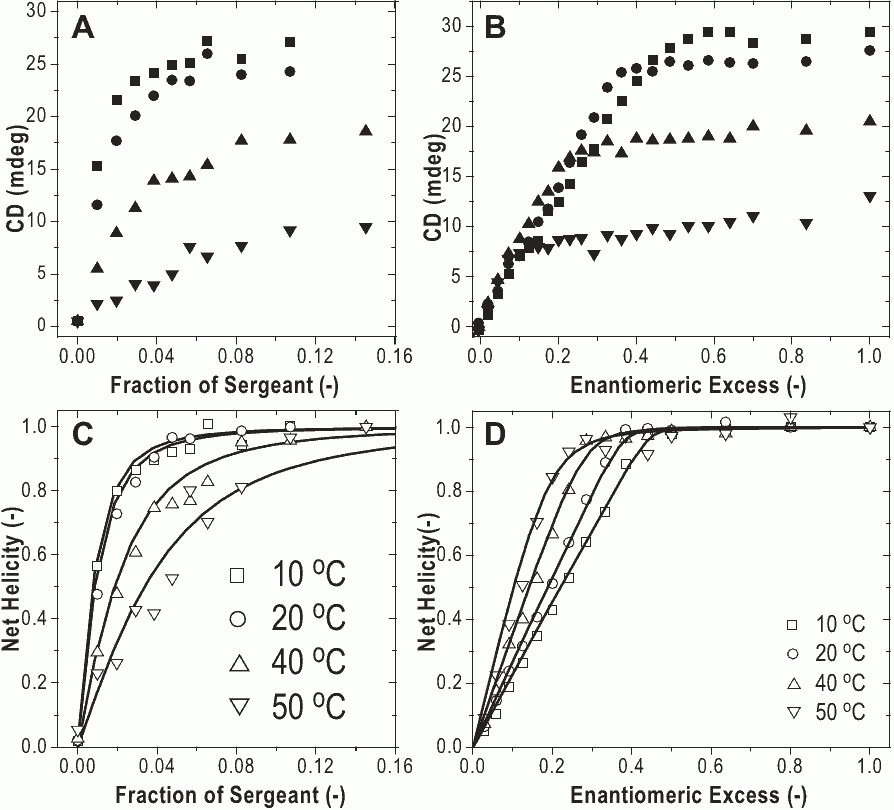
\includegraphics[width=1\textwidth]{sec2/temp.png}}}\end{figure}\end{columns}
\end{frame}


\subsubsection{Regola di maggioranza}\begin{frame}\frametitle{Amplificazione di chiralità}\framesubtitle{Regola di maggioranza}
\begin{columns}
\column{0.64\linewidth}\textbf{Per avere una maggiore amplificazione chirale in esp. regola di maggioranza} si può diminuire la \textbf{penalità per errore} ma non troppo: esiste un valore \textbf{ottimale}. Infatti una penalità=0 significherebbe che la chiralità non viene più espressa ad un livello supramolecolare.

Con un valore \textbf{maggiore della penalità per inversione} di elica si ha un valore minore dell'ottimo di penalità per errore ed un \textbf{minore e.e. a cui si avrà omochiralità} supramolecolare. \cite{tesi}
\column{0.36\linewidth}\vspace{-13pt}
\begin{figure}{\centering{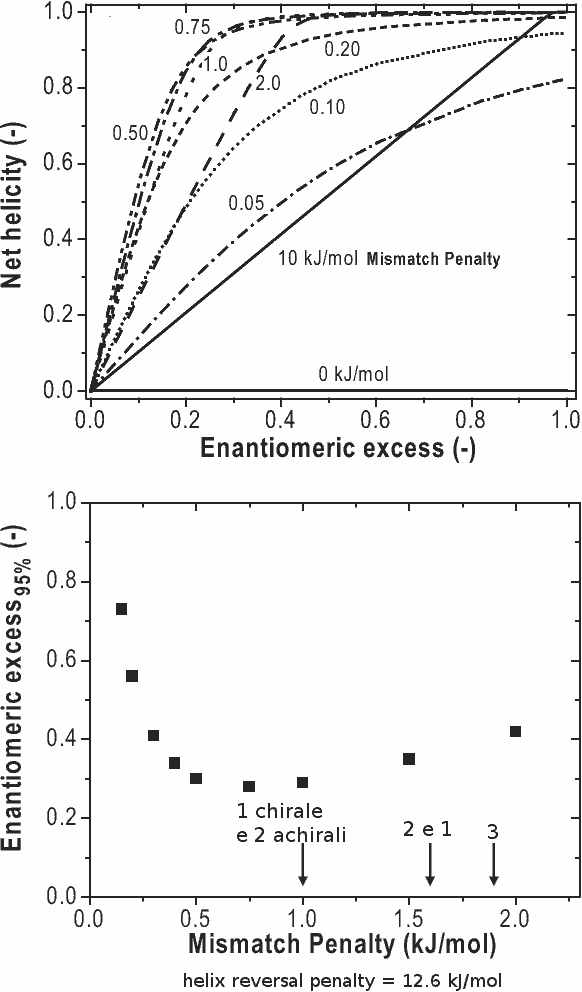
\includegraphics[width=1\textwidth]{sec2/maggioranza-ottimo.png}}}\end{figure}
\end{columns}
\end{frame}
\logo{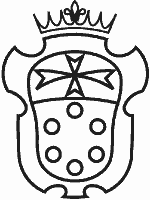
\includegraphics[width=0.07\paperwidth]{snslogo.png}}

\subsection{Altre unità discotiche}\begin{frame}\frametitle{Altre unità discotiche}
\begin{columns}
\column{0.4\linewidth}
\begin{figure}{\centering{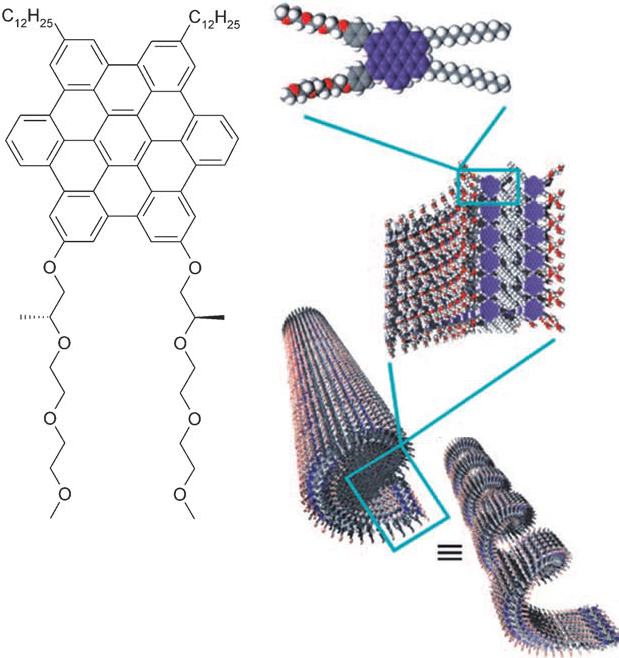
\includegraphics[width=1\textwidth]{sec2/coronene.png}}}\end{figure}
Forte \textbf{amplificazione} di chiralità.
\column{0.6\linewidth}\begin{columns}
\column{0.6\linewidth}
\begin{figure}{\centering{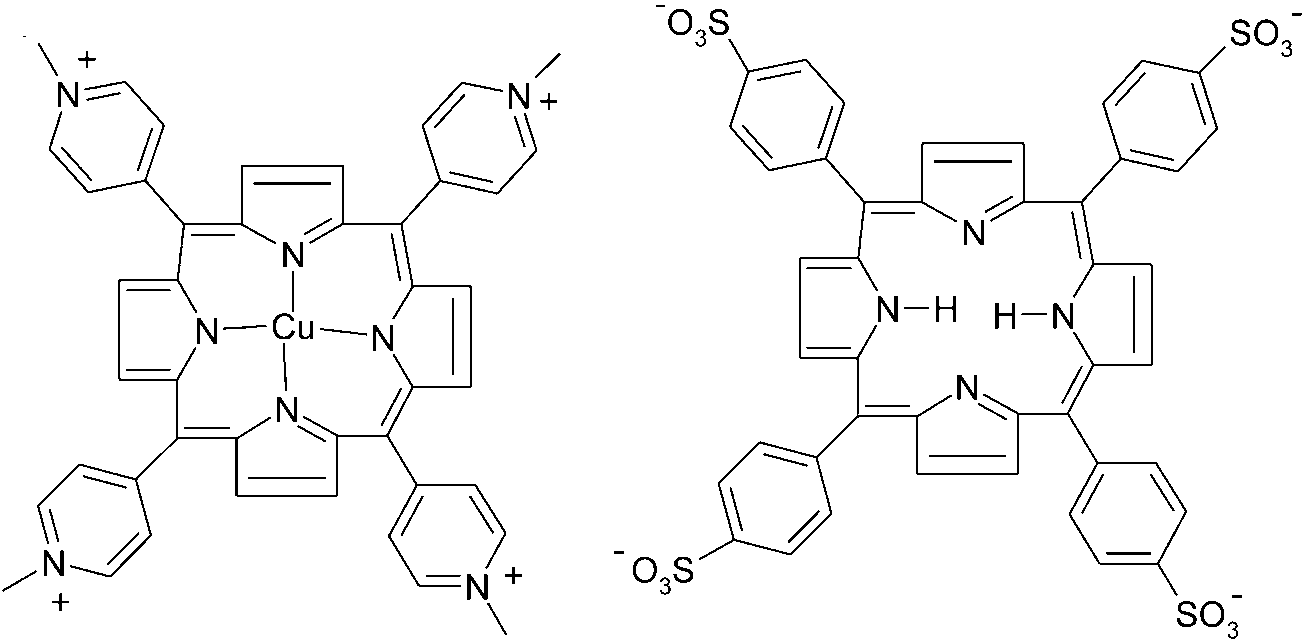
\includegraphics[width=1\textwidth]{sec2/porfirine.png}}}\end{figure}
\column{0.4\linewidth}Spontaneamente in eliche, \textbf{memorizzano la chiralità} dal templato di poliglutammato.\end{columns}
\begin{columns}
\column{0.6\linewidth}\begin{figure}{\centering{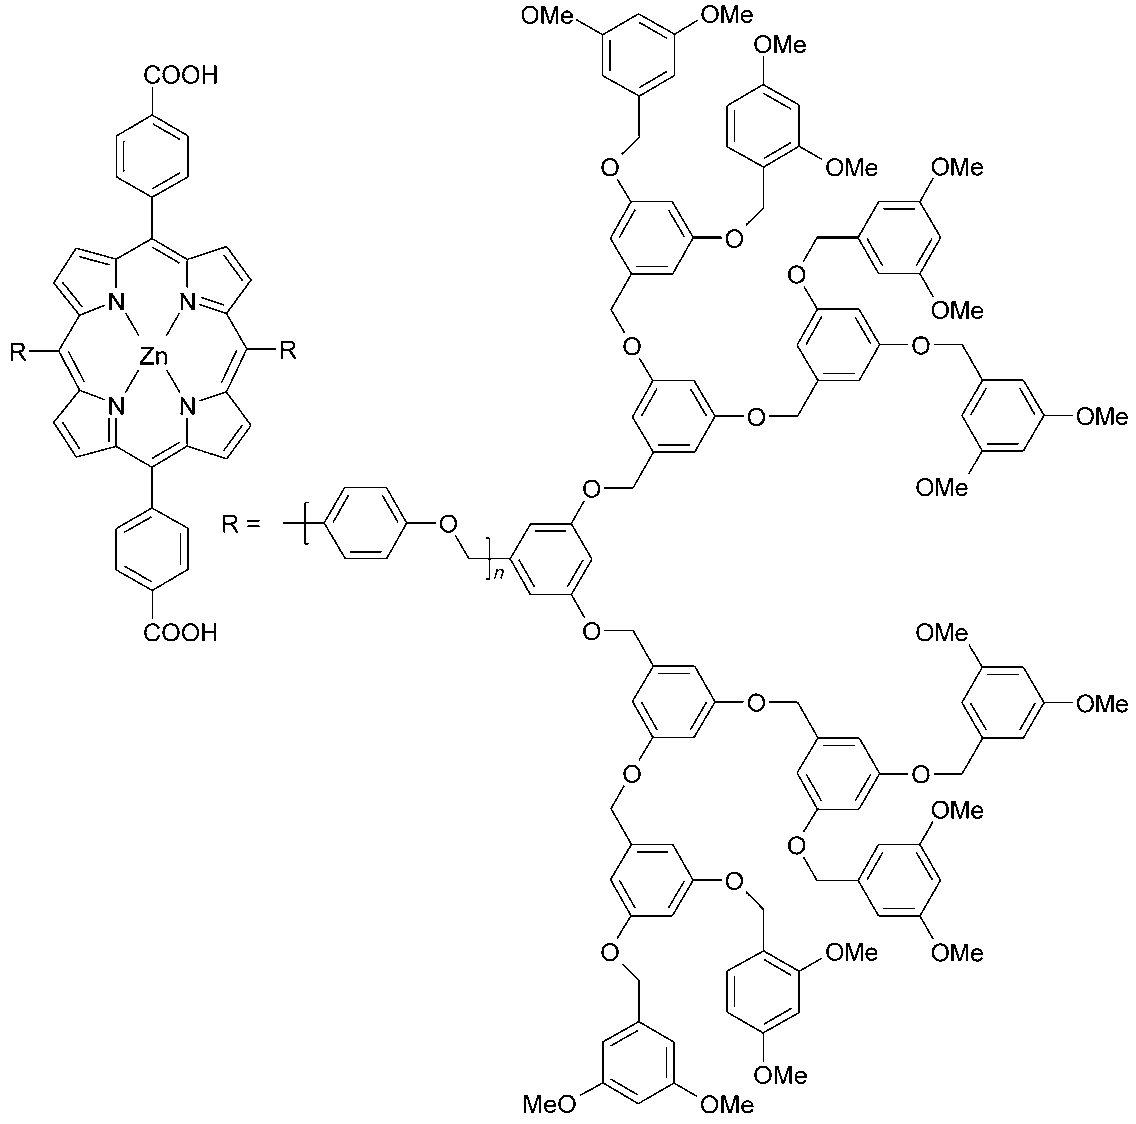
\includegraphics[width=1\textwidth]{sec2/zinco-dendritico.png}}}\end{figure}\column{0.4\linewidth}
Induzione di chiralità dalla \textbf{direzione dello spin-coating}.
\end{columns}\end{columns}
\end{frame}
